% ---------------------------------------------------------------------------------------------------------------
% TEMPLATE PARA TRABALHO DE CONCLUSÃO DE CURSO
% Universidade Tecnológica Federal do Paraná - UTFPR
% Customização da classe abnTeX2 (http://www.abntex.net.br/) para as normas da UTFPR
%
% Autores: Diego Marczal
% 	       Michael Vornes <https://github.com/mvornes>
% Adaptação (DACOM-CP): Silvio Ricardo Rodrigues Sanches
%
%----------------------------------------------------------------------------------------------------------------
% Codificação: UTF-8
% LaTeX:  abnTeX2          
% ---------------------------------------------------------------------------------------------------------------


% CARREGA CLASSE PERSONALIZADA DA UTFPR--------------------------------------------------------------------------
\documentclass[%twoside,                   % Impressão em frente e verso
    	        oneside,                   % Impressão apenas frente
]{configuracoes/utfpr-abntex2}


% INCLUI ARQUIVOS DE CONFIGURAÇÕES-------------------------------------------------------------------------------
% REFERÊNCIAS------------------------------------------------------------------
\usepackage[%
    alf,
    abnt-emphasize=bf,
    bibjustif,
    recuo=0cm,
    abnt-url-package=url,       % Utiliza o pacote url
    abnt-refinfo=yes,           % Utiliza o estilo bibliográfico abnt-refinfo
    abnt-etal-cite=3,
    abnt-etal-list=3,
    abnt-thesis-year=final
]{abntex2cite}                  % Configura as citações bibliográficas conforme a norma ABNT

% PACOTES----------------------------------------------------------------------
\usepackage[utf8]{inputenc}                                 % Codificação do documento
\usepackage[T1]{fontenc}                                    % Seleção de código de fonte
\usepackage{booktabs}                                       % Réguas horizontais em tabelas
\usepackage{color, colortbl}                                % Controle das cores
\usepackage{float}                                          % Necessário para tabelas/figuras em ambiente multi-colunas
\usepackage{graphicx}                                       % Inclusão de gráficos e figuras
\usepackage{icomma}                                         % Uso de vírgulas em expressões matemáticas
\usepackage{indentfirst}                                    % Indenta o primeiro parágrafo de cada seção
\usepackage{microtype}                                      % Melhora a justificação do documento
\usepackage{multirow, array}                                % Permite tabelas com múltiplas linhas e colunas
\usepackage{subeqnarray}                                    % Permite subnumeração de equações
\usepackage{lastpage}                                       % Para encontrar última página do documento
\usepackage{verbatim}                                       % Permite apresentar texto tal como escrito no documento, ainda que sejam comandos Latex
\usepackage{amsfonts, amssymb, amsmath}                     % Fontes e símbolos matemáticos
\usepackage[algoruled, portuguese]{algorithm2e}             % Permite escrever algoritmos em português
%\usepackage[scaled]{helvet}                                % Usa a fonte Helvetica
\usepackage{times}                                          % Usa a fonte Times
%\usepackage{palatino}                                      % Usa a fonte Palatino
%\usepackage{lmodern}                                       % Usa a fonte Latin Modern
\usepackage[bottom]{footmisc}                               % Mantém as notas de rodapé sempre na mesma posição
\usepackage{ae, aecompl}                                    % Fontes de alta qualidade
\usepackage{latexsym}                                       % Símbolos matemáticos
\usepackage{lscape}                                         % Permite páginas em modo "paisagem"
%\usepackage{picinpar}                                      % Dispor imagens em parágrafos
%\usepackage{scalefnt}                                      % Permite redimensionar tamanho da fonte
%\usepackage{subfig}                                        % Posicionamento de figuras
%\usepackage{upgreek}                                       % Fonte letras gregas

% Redefine a fonte para uma fonte similar a Arial (fonte Helvetica)
\renewcommand*\familydefault{\sfdefault}

% CONFIGURAÇÕES DE APARÊNCIA DO PDF FINAL--------------------------------------
\makeatletter
\hypersetup{%
    portuguese,
    colorlinks=true,   % true: "links" coloridos; false: "links" em caixas de texto
    linkcolor=blue,    % Define cor dos "links" internos
    citecolor=blue,    % Define cor dos "links" para as referências bibliográficas
    filecolor=blue,    % Define cor dos "links" para arquivos
    urlcolor=blue,     % Define a cor dos "hiperlinks"
    breaklinks=true,
    pdftitle={\@title},
    pdfauthor={\@author},
    pdfkeywords={abnt, latex, abntex, abntex2}
}
\makeatother

% ALTERA O ASPECTO DA COR AZUL--------------------------------------------------
\definecolor{blue}{RGB}{41,5,195}

% REDEFINIÇÃO DE LABELS---------------------------------------------------------
\renewcommand{\algorithmautorefname}{Algoritmo}
\def\equationautorefname~#1\null{Equa\c c\~ao~(#1)\null}

% CRIA ÍNDICE REMISSIVO---------------------------------------------------------
\makeindex

% HIFENIZAÇÃO DE PALAVRAS QUE NÃO ESTÃO NO DICIONÁRIO---------------------------
\hyphenation{%
    qua-dros-cha-ve
    Kat-sa-gge-los
}



% INCLUI ARQUIVOS DO TRABALHO DE CONCLUSÃO DE CURSO (PRÉ-TEXTUAIS, TEXTUAIS, PÓS-TEXTUAIS)-----------------------

% INSERE CAPA E FOLHA DE ROSTO
% CAPA---------------------------------------------------------------------------------------------------

% ORIENTAÇÕES GERAIS-------------------------------------------------------------------------------------
% Caso algum dos campos não se aplique ao seu trabalho, como por exemplo,
% se não houve coorientador, apenas deixe vazio.
% Exemplos: 
% \coorientador{}
% \departamento{}

% DADOS DO TRABALHO--------------------------------------------------------------------------------------
\titulo{Título do Trabalho: Subtítulo do Trabalho}
\titleabstract{Title in English}
\autor{Nome Completo do Autor}
\autorcitacao{SOBRENOME, Nome} % Sobrenome em maiúsculo
\local{Cornélio Procópio}
\data{2018}

% NATUREZA DO TRABALHO-----------------------------------------------------------------------------------
% Opções: 
% - Trabalho de Conclusão de Curso (se for Graduação)
% - Dissertação (se for Mestrado)
% - Tese (se for Doutorado)
% - Projeto de Qualificação (se for Mestrado ou Doutorado)
\projeto{Trabalho de Conclusão de Curso}

% TÍTULO ACADÊMICO---------------------------------------------------------------------------------------
% Opções:
% - Bacharel ou Tecnólogo (Se a natureza for Trabalho de Conclusão de Curso)
% - Mestre (Se a natureza for Dissertação)
% - Doutor (Se a natureza for Tese)
% - Mestre ou Doutor (Se a natureza for Projeto de Qualificação)
\tituloAcademico{...}

% ÁREA DE CONCENTRAÇÃO E LINHA DE PESQUISA---------------------------------------------------------------
% Se a natureza for Trabalho de Conclusão de Curso, deixe ambos os campos vazios
% Se for programa de Pós-graduação, indique a área de concentração e a linha de pesquisa
\areaconcentracao{}
\linhapesquisa{}

% DADOS DA INSTITUIÇÃO-----------------------------------------------------------------------------------
% Se a natureza for Trabalho de Conclusão de Curso, coloque o nome do curso de graduação em "programa"
% Formato para o logo da Instituição: \logoinstituicao{<escala>}{<caminho/nome do arquivo>}
\instituicao{Universidade Tecnológica Federal do Paraná}
\departamento{Departamento Acadêmico de Computação}
\programa{Curso de Engenharia de Computação}
\logoinstituicao{0.2}{dados/figuras/logo-instituicao.png} 

% DADOS DOS ORIENTADORES---------------------------------------------------------------------------------
\orientador{Prof. Dr. Claiton de Oliveira}
%\orientador[Orientadora:]{Nome da orientadora}
\instOrientador{Universidade Tecnológica Federal do Paraná}

\coorientador{Prof. Dr. Pedro Henrique Bugatti}
%\coorientador[Coorientadora:]{Nome da coorientadora}
\instCoorientador{Instituição do coorientador}

% FOLHA DE ROSTO--------------------------------------------------------------------------------------------------------

% TRABALHO DE CONCLUSÃO DE CURSO
 \preambulo{{\imprimirprojeto} apresentado ao {\imprimirprograma} da {\imprimirinstituicao}, como requisito parcial para a obtenção do título de {\imprimirtituloAcademico}.}

% DISSERTAÇÃO DE MESTRADO
% \preambulo{{\imprimirprojeto} apresentada ao Programa de \mbox{Pós-graduação} da {\imprimirinstituicao}, como requisito parcial para obtenção do título de {\imprimirtituloAcademico}.}

% TESE DE DOUTORADO
% \preambulo{{\imprimirprojeto} apresentada ao Programa de \mbox{Pós-graduação} da {\imprimirinstituicao}, como requisito parcial para a obtenção do título de {\imprimirtituloAcademico}.}

% PROJETO DE QUALIFICAÇÃO DE MESTRADO OU DOUTORADO
%\preambulo{{\imprimirprojeto} apresentado ao Programa de \mbox{Pós-graduação} da {\imprimirinstituicao}, como requisito parcial para a obtenção do título de {\imprimirtituloAcademico}.}

% OBSERVAÇÕES-----------------------------------------------------------------------------------------------------------
% Altere este arquivo APENAS comentando as linhas que não se aplicam ao tipo de trabalho acadêmico desejado.


\begin{document}

\pretextual
\imprimircapa                                               	           % Comando para imprimir Capa
\imprimirfolhaderosto{}                                     		   % Comando para imprimir Folha de rosto
% INSERE ELEMENTOS PRÉ-TEXTUAIS
% DEDICATÓRIA------------------------------------------------------------------

\renewcommand{\dedicatorianame}{DEDICATÓRIA}

\begin{dedicatoria}

Altere este texto inserindo a dedicatória do seu trabalho. 

\end{dedicatoria}
          			   % Dedicatória
% AGRADECIMENTOS---------------------------------------------------------------

\begin{agradecimentos}[AGRADECIMENTOS]

Edite e coloque aqui os agradecimentos às pessoas e/ou instituições que contribuíram para a realização do trabalho.

É obrigatório o agradecimento às instituições de fomento à pesquisa que financiaram total ou parcialmente o trabalho, inclusive no que diz respeito à concessão de bolsas.

\end{agradecimentos}
        			   % Agradecimentos
% EPÍGRAFE---------------------------------------------------------------------

\renewcommand{\epigraphname}{EPÍGRAFE}

\begin{epigrafe}

\textit{Eu denomino meu campo de Gestão do Conhecimento, mas você não pode gerenciar conhecimento. Ninguém pode. O que pode fazer - o que a empresa pode fazer - é gerenciar o ambiente que otimize o conhecimento. (PRUSAK, Laurence, 1997).}

\end{epigrafe}

% OBSERVAÇÕES------------------------------------------------------------------
% Altere o texto para inserir a epígrafe do seu trabalho
              			   % Epígrafe
% RESUMO--------------------------------------------------------------------------------

\begin{resumo}[RESUMO]
\begin{SingleSpacing}

% Não altere esta seção do texto--------------------------------------------------------
\imprimirautorcitacao. \imprimirtitulo. \imprimirdata. \pageref {LastPage} f. \imprimirprojeto\ – \imprimirprograma, \imprimirinstituicao. \imprimirlocal, \imprimirdata.\\
%---------------------------------------------------------------------------------------

O Resumo é um elemento obrigatório em tese, dissertação, monografia e TCC, constituído de uma seqüência de frases concisas e objetivas, fornecendo uma visão rápida e clara do conteúdo do estudo. O texto deverá conter no máximo 500 palavras e ser antecedido
pela referência do estudo. Também, não deve conter citações. O resumo deve ser redigido em parágrafo único, espaçamento simples e seguido das palavras representativas do conteúdo do estudo, isto é, palavras-chave, em número de três a cinco, separadas entre si por ponto e finalizadas também por ponto. Usar o verbo na terceira pessoa do singular, com linguagem impessoal, bem como fazer uso, preferencialmente, da voz ativa. Texto contendo um único parágrafo.\\

\textbf{Palavras-chave}: Palavra. Segunda Palavra. Outra palavra.

\end{SingleSpacing}
\end{resumo}

% OBSERVAÇÕES---------------------------------------------------------------------------
% Altere o texto inserindo o Resumo do seu trabalho.
% Escolha de 3 a 5 palavras ou termos que descrevam bem o seu trabalho 
             			   % Resumo em Português
% ABSTRACT--------------------------------------------------------------------------------

\begin{resumo}[ABSTRACT]
\begin{SingleSpacing}

% Não altere esta seção do texto--------------------------------------------------------
\imprimirautorcitacao. \imprimirtitleabstract. \imprimirdata. \pageref {LastPage} f. \imprimirprojeto\ – \imprimirprograma, \imprimirinstituicao. \imprimirlocal, \imprimirdata.\\
%---------------------------------------------------------------------------------------

Elemento obrigatório em tese, dissertação, monografia e TCC. É a versão do resumo em português para o idioma de divulgação internacional. Deve ser antecedido pela referência do estudo. Deve aparecer em folha distinta do resumo em língua portuguesa e seguido das palavras representativas do conteúdo do estudo, isto é, das palavras-chave. Sugere-se a elaboração do resumo (Abstract) e das palavras-chave (Keywords) em inglês; para resumos em outras línguas, que não o inglês, consultar o departamento / curso de origem.\\

\textbf{Keywords}: Word. Second Word. Another word.

\end{SingleSpacing}
\end{resumo}

% OBSERVAÇÕES---------------------------------------------------------------------------
% Altere o texto inserindo o Abstract do seu trabalho.
% Escolha de 3 a 5 palavras ou termos que descrevam bem o seu trabalho 
             		           % Resumo em Inglês
% Lista de Figuras----------------------------------------------------------------

\pdfbookmark[0]{\listfigurename}{lof}
\listoffigures*
\cleardoublepage

% OBSERVAÇÕES---------------------------------------------------------------------
% Este arquivo não precisa de ser alterado, pois a lista é gerada automaticamente.
   % Lista de Figuras
% LISTA DE QUADROS----------------------------------------------------------------

\renewcommand{\listofquadrosname}{LISTA DE QUADROS}

\pdfbookmark[0]{\listofquadrosname}{loq}
\listofquadros*
\cleardoublepage

% OBSERVAÇÕES---------------------------------------------------------------------
% Este arquivo não necessita de ser editado. A lista é gerada automaticamente.
   % Lista de Quadros
% LISTA DE TABELAS-------------------------------------------------------------

\pdfbookmark[0]{\listtablename}{lot}
\listoftables*
\cleardoublepage

% OBSERVAÇÕES-------------------------------------------------------------------
% Este arquivo não precisa ser alterado, pois a lista é gerada automaticamente.
         		   % Lista de Tabelas
% LISTA DE ABREVIATURAS E SIGLAS----------------------------------------------------------

\begin{siglas}
    \item[ABNT] Associação Brasileira de Normas Técnicas
    \item[DECOM] Departamento de Computação
\end{siglas}

% OBSERVAÇÕES-----------------------------------------------------------------------------
% Altere a lista acima para definir os acrônimos e siglas utilizados neste trabalho
          		   % Lista de Abreviaturas e Siglas
% LISTA DE SÍMBOLOS------------------------------------------------------------

\begin{simbolos}
    \item[$ \Gamma $] Letra grega Gama
    \item[$ \lambda $] Comprimento de onda
    \item[$ \in $] Pertence
\end{simbolos}

% OBSERVAÇÕES-------------------------------------------------------------------
% Altere a lista acima para definir os símbolos utilizados no trabalho
        		   % Lista de Símbolos
% LISTA DE ALGORITMOS----------------------------------------------------------

\newcommand{\algoritmoname}{Algoritmo}
\renewcommand{\listalgorithmcfname}{LISTA DE ALGORITMOS}

\floatname{algocf}{\algoritmoname}
\newlistof{listofalgoritmos}{loa}{\listalgoritmoname}
\newlistentry{algocf}{loa}{0}

\counterwithout{algocf}{chapter}
\renewcommand{\cftalgocfname}{\algoritmoname\space}
\renewcommand*{\cftalgocfaftersnum}{\hfill--\hfill}

\pdfbookmark[0]{\listalgorithmcfname}{loa}
\listofalgorithms
\cleardoublepage

% OBSERVAÇÕES------------------------------------------------------------------
% Este arquivo não precisa ser alterado, pois a lista é gerada automaticamente.
   % Lista de Algoritmos
% SUMÁRIO----------------------------------------------------------------------

\renewcommand{\contentsname}{SUMÁRIO}

\pdfbookmark[0]{\contentsname}{toc}
\tableofcontents*
\cleardoublepage

% OBSERVAÇÕES-------------------------------------------------------------------
% Este arquivo não precisa ser alterado, pois o sumário é gerado automaticamente.
               			   % Sumário

\textual
% INSERE ELEMENTOS TEXTUAIS
% INTRODUÇÃO-------------------------------------------------------------------

\chapter{INTRODUÇÃO}
\label{chap:introducao}

Edite e coloque aqui o seu texto de introdução.

A Introdução é a parte inicial do texto, na qual devem constar o tema e a delimitação do assunto tratado, objetivos da pesquisa e outros elementos necessários para situar o tema do trabalho, tais como: justificativa, procedimentos metodológicos (classificação inicial), embasamento teórico (principais bases sintetizadas) e estrutura do trabalho, tratados de forma sucinta. Recursos utilizados e cronograma são incluídos quando necessário. Salienta-se que os procedimentos metodológicos e o embasamento teórico são tratados, posteriormente, em capítulos próprios e com a profundidade necessária ao trabalho de pesquisa.

\section{CONSIDERAÇÕES INICIAIS}
\label{sec:consideracoesIniciais}

Este documento é um \emph{template} \LaTeX{} que foi concebido, primariamente, para ser utilizado na elaboração de Trabalho de Conclusão de Curs em conformidade com as normas da Universidade Tecnológica Federal do Paraná.

Para a produção deste \emph{template} foi necessário adaptar o arquivo {\ttfamily abntex2.cls}. Assim, foi produzido o arquivo {\ttfamily utfpr-abntex2.cls} que define o \verb|documentclass| específico para a UTFPR.

Antes de começar a escrever o seu trabalho acadêmico utilizando este \emph{template}, é importante saber que há dois arquivos que você precisará editar para que a capa e a folha de rosto de seu trabalho sejam geradas automaticamente.
São eles os arquivos {\ttfamily capa.tex} e {\ttfamily folha-rosto.tex}, ambos no diretório  {\ttfamily /elementos-pre-textuais}.
No arquivo {\ttfamily capa.tex} deverá ser informado nome do autor, título do trabalho, natureza do trabalho, nome do orientador e outras informações necessárias.
No arquivo {\ttfamily folha-rosto.tex}, que contém o texto padrão estabelecendo que este documento é um requisito parcial para a obtenção do título pretendido, será necessário apenas comentar as linhas que não se aplicam ao tipo de trabalho acadêmico.

A compilação para gerar um arquivo no formato pdf, incluindo corretamente as referências bibliográficas, deve ser realizada utilizando o comando \verb|makefile|, disponível na mesma pasta onde está o arquivo principal \verb|utfpr-tcc.tex|. Caso seja alterado o nome do arquivo \verb|utfpr-tcc.tex|, deverá ser alterado no arquivo \verb|makefile| também.

\section{OBJETIVOS}
\label{sec:objetivos}

\section{ORGANIZAÇÃO DO TRABALHO}
\label{sec:organizacaoTrabalho}

Normalmente ao final da introdução é apresentada, em um ou dois parágrafos curtos, a organização do restante do trabalho acadêmico.
Deve-se dizer o quê será apresentado em cada um dos demais capítulos.
                		           % Introdução
% FUNDAMENTAÇÃO TEÓRICA--------------------------------------------------------

\chapter{FUNDAMENTAÇÃO TEÓRICA}
\label{chap:fundamentacaoTeorica}

As grandes habilidades do ser humano, como a capacidade de aprendizado e de realizar funções complexas, motivam muitos pesquisadores a investigar o funcionamento do cérebro e desenvolverem técnicas que possibilitem reproduzir suas
funções (FERNEDA, 2006). Motivados a tornar possível que computadores executem tarefas consideradas complexas, ao longo dos anos, foram propostos diversos algoritmos capazes de realizar tarefas como reconhecimento de sinais de áudios e imagens, tomada de decisão, entre outros, de maneira eficaz e eficiente. Paradigmas que buscam reproduzir as funções do cérebro humano compreendem a área de Inteligência Artificial – IA – da ciência da computação.

\section{APRENDIZADO DE MÁQUINA}
\label{sec:titSecAprenMaquina}

Aprendizado de máquina – AM – é uma subárea de grande importância da Inteligência Artificial, pois o aprendizado é um fator fundamental para um comportamento inteligente (BATISTA, 2003, p. 39). A construção do seu modelo matemático foi baseado no funcionamento dos neurônios do cérebro dos vertebrados, o qual denomina-se pela técnica computacional de Rede Neural Artificial, que adquirem conhecimento com base em experiências, melhorando gradualmente sua capacidade de desempenho.

O AM tem o objetivo de construir programas computacionais que sejam capazes de obter conhecimento de maneira autônoma, ou seja, desenvolver sistemas que baseiam tomadas de decisões em experiências adquiridas anteriormente, por meio de resoluções bem sucedidas de problemas semelhantes (MONARD; BARANAUSKAS, 2003).

O uso de algoritmos de aprendizado permitiu que diversas tarefas complexas fossem possíveis de serem realizadas e até superar os resultados obtidos por humanos. Um exemplo é um algoritmo de aprendizado de máquina, desenvolvido por Silver et al. (2016), que venceu o campeão mundial do jogo \textit{Go}, um dos jogos estratégicos mais antigos do mundo que possui uma alta complexidade e uma infinidade de possibilidades de jogadas.

O algoritmo de AM também permitiu que tarefas complexas ou exaustivas para o humano fossem realizadas de forma eficiênte. Como em Souto et al. (2003), por exemplo, um algoritmo de aprendizado de máquina foi utilizado para realizar a análise de dados biológicos, dada a restrição da análise manual diante do número de dados biológicos que aumenta exponencialmente a cada ano.


\subsection{APRENDIZADO SUPERVISIONADO}
\label{sec:titSecAprenSupervisionado}

A indução é um conceito que caracteriza a forma de obter conclusões genéricas com base em exemplos específicos, em outras palavras, o aprendizado ocorre à partir de uma inferência em padrões apresentados. A indução é umas das principais formas de derivar conhecimento novo, foi com ela que as principais descobertas do mundo tornaram-se conhecidas. Embora a indução seja uma das principais maneiras do cérebro humano converter exemplos em conhecimento, deve-se ter cuidado ao utilizá-la, pois com padrões insuficientes ou mal escolhidos levam a uma inferência incorreta (MONARD; BARANAUSKAS, 2003, cap. 4).	

Além de uma subárea do aprendizado de máquina, existem duas vertentes básicas de aprendizado indutivo, o aprendizado supervisionado e o não supervisionado. O presente trabalho abordou o aprendizado supervisionado.

O aprendizado supervisionado, ou indutor, consiste em apresentar a um algoritmo dados de treinamento que representam alguns padrões de entrada e seus respectivos padrões de saída esperados, ou seja, o algoritmo conhece a priori o rótulo de todo o conjunto de dados de treinamento (BLASCHKO; KUMAR; TASKAR, 2013). Dessa forma, o mesmo consegue, a partir de tais dados construir um modelo de aprendizado capaz de ser utilizado posteriormente para rotular amostras desconhecidas (i.e. amostras de teste). Recentemente, o aprendizado supervisionado baseado em arquiteturas de redes neurais profundas, ressurgiu apresentando resultados notáveis quando aplicados a problemas que envolvam visão computacional e análise de imagens, sendo utilizado em aplicações como classificação de imagens e/ou detecção de objetos (KRIZHEVSKY; SUTSKEVER; HINTON, 2012).


\subsection{APRENDIZADO PROFUNDO}
\label{sec:titSecAprenProfundo}

Aprendizado profundo, do inglês \textit{Deep Learning} (DL), é uma subárea do aprendizado de máquina que explora o processamento de informações em diversos estágios, com o objetivo de classificar padrões e realizar a aprendizagem de recurso ou representação (WAN et al., 2014). A modelagem do problema de reconhecimento é feita por meio de um grafo ponderado em camadas, cada camada possui um conjunto de características abstratas que são conectadas as características das demais camadas (CHEN et al., 2015).

As principais áreas de pesquisa do aprendizado profundo são no desenvolvimento de técnicas capazes de reproduzir alguns comportamentos humanos, como processamento de linguagem natural, reconhecimento visual e reconhecimento da fala. A DL é muito utilizada nessas áreas por ser uma tecnologia que possibilita aprendizado ininterrupto, semelhante ao cérebro humano, além de possuir grande flexibilidade e capacidade de processamento de informações complexas. Comparada a outras metodologias clássicas de aprendizado de máquina, o aprendizado profundo oferece grandes vantagens, podendo superar a capacidade humana, principalmente na resolução de problemas com um grande volume de dados não estruturado. Isso ocorre devido ao fato do seu modelo matemático ser mais flexível, isso possibilita que os \textit{inputs} sejam definidos pelo modelo, no qual analisa todos os parâmetros de entrada e decide quais trarão os melhores resultados (FERNANDES; SILVA, 2017).

LeCun et al. (2015) acreditam que em um futuro próximo o aprendizado de máquina será cada vez mais utilizado por demandar pouco trabalho manual para a sua construção, podendo usufruir de uma melhor maneira da capacidade computacional e de dados.

\section{IMAGENS NA VISÃO COMPUTACIONAL}
\label{sec:titSecVisaoComputacional}

A visão computacional tornou-se grande aliada para solucionar problemas do homem. Um grande exemplo são os radares fixos de velocidade, quando um carro cruzar entre os sensores localizados no asfalto, acima de uma velocidade pré-determinada, é acionada uma câmera, essa câmera captura uma imagem da placa traseira de um automóvel e em seguida é identificado cada caractere da placa. Todo o processo de identificar uma placa na traseira de um automóvel e reconhecer os sete caracteres da placa envolve processamento digital de imagem.

Processamento Digital de Imagens (PDI) trata-se de processar sinais com o intuito de extrair mais facilmente as informações contida (ALBUQUERQUE, 2003). O processamento envolve algumas etapas, como: aquisição da imagem, pré-processamento, segmentação, representação e descrição, e reconhecimento e interpretação (PEDRINI; SCHWARTZ, 2008).

A etapa de aquisição, como o próprio nome induz, refere-se a adquirir uma imagem. O pré-processamento refere-se à algumas técnicas que serão empregadas na imagem de modo a obter melhores resultados na extração das informações desejadas, por exemplo, na \autoref{fig:figura-exemploPreProcessamento} (a) apresenta um raio-x com pouca visibilidade dos ossos presentes  e (b) a imagem após aplicação do filtro de equalização de histograma. O processo de segmentação objetiva extrair os objetos de interesse da imagem, frequentemente usada para remoção de fundos. Em representação e descrição serão extraídas atributos da imagem, essa etapa é caracterizada pela rotulação, onde será atribuído uma \textit{label} que poderá indicar a qual classe a imagem pertence; e pela extração de atributos onde será reunido um conjunto de características, representadas numericamente, que podem descrever cores, texturas, formas, entre outras.  A última etapa, reconhecimento e interpretação, objetiva realizar de, maneira automática, a identificação dos objetos segmentados. Nessa última etapa é comum o uso de uma sub-área da IA, o aprendizado de máquina, pela necessidade de realizar um aprendizado e uma representação dos padrões aprendidos (ALBUQUERQUE, 2003).


\begin{figure}[!htb]
    \centering
    \caption{Exemplo de pré-processamento}
    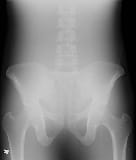
\includegraphics[width=0.3\textwidth]{./dados/figuras/figura1-a.jpg}
    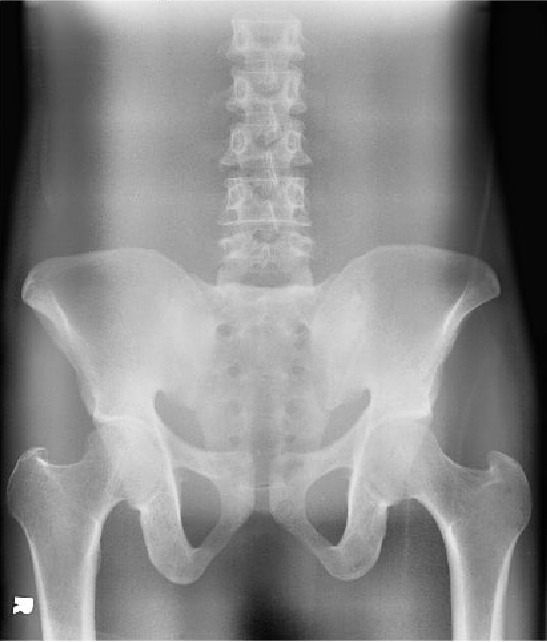
\includegraphics[width=0.3\textwidth]{./dados/figuras/figura1-b.jpeg}
    \fonte{Adaptado de}
    \label{fig:figura-exemploPreProcessamento}
\end{figure}


\section{ANÁLISE DE SEMENTES}
\label{sec:titSecAnalSementes}

O Brasil é o maior produtor e exportador de soja do mundo, são inúmeras as vantagens que o levaram a essa posição, como a alta capacidade do grão em se adaptar a diferentes tipos de solo e clima. Isso exige que a produção seja sempre de alta qualidade, garantir um alto vigor à soja garante que o grão possa tolerar facilmente mudanças climáticas, doenças e pragas, por exemplo (HORIKOSHI et al., 2018).

Existem diversos testes e experimentos em laboratórios que pesquisam e aplicam técnicas para evolução da qualidade do grão. Um teste em destaque é o teste de tetrazólio, um método de controle de qualidade, com alta precisão, rapidez e possibilidade de extrair uma grande quantidade de informações. O teste permite verificar o vigor do grão de soja e possíveis causas que o levaram a ter o vigor reduzido, como dano por excesso de umidade, danos mecânicos ou danos causados por percevejos (PAGLIONE, 2016).

\begin{figure}[!htb]
    \centering
    \caption{Sementes submetidas ao teste de tetrazólio}
    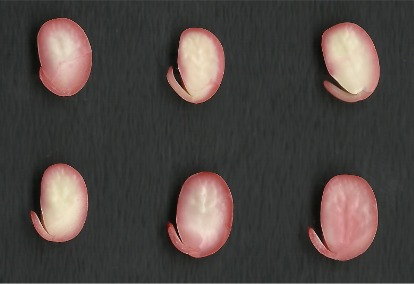
\includegraphics[width=0.5\textwidth]{./dados/figuras/soybean.jpeg}
    \fonte{(SANTANNA et al., 2014)}
    \label{fig:figura-sojasTeste}
\end{figure}

O teste consiste em aplicar uma solução em uma amostra de sementes, que foram previamente cortadas longitudinal e medianamente, no sentido do comprimento, selecionando a metade mais apropriada ao teste (OLIVEIRA, 2009). A solução do teste proporciona aos grãos amostras uma cor avermelhada, segundo França Neto et al. (1998), as diferentes cores observadas são características que são consideradas nos resultados do teste. Por exemplo, a cor rosa claro sinaliza uma semente de alto vigor, por outro lado, sementes que apresentam uma cor rosa escuro apresentam tecido em deterioração.

         % Revisão de Literatura
% PLANO DE TRABALHO------------------------------------------------------------------

\chapter{PLANO DE TRABALHO}
\label{chap:metodologia}
Alguns conceitos de processamento de imagens foram apresentados até o momento, bem como algumas técnicas de inteligência artificial que podem ser utilizadas na etapa de reconhecimento e interpretação. 

A proposta deste trabalho visa a utilização de metodologias de aprendizado de máquina, sendo aplicado conceitos de aprendizado profundo supervisionado, de maneira a reduzir tempo de processamento e obter um aumento nos resultados de acurácia a partir de resultados apresentados por \citeonline{Paglione2016}. Em seu trabalho, \citeonline{Paglione2016} apresenta uma proposta de melhoria em resultados de acurácia e tempo para o teste de tetrazólio utilizando técnicas de PDI, por meio de diferentes métodos de segmentação de imagem.

\section{METODOLOGIA PROPOSTA}
\label{sec:titSecMetProposta}

Para o presente trabalho será utilizado uma base de imagens de sementes de soja provenientes do trabalho desenvolvido por \citeonline{Santanna2014}. Porém serão aplicadas técnicas de processamento de imagem propostos por \citeonline{Paglione2016}, o \textit{pipele} de execução é apresentado na \autoref{fig:figura-pipelinePreProcessamento}, das quais mostraram resultados otimizados em relação ao trabalho apresentado por \citeonline{Santanna2014}.

\begin{figure}[!htb]
    \centering
    \caption{Pipeline do pré-processamento}
    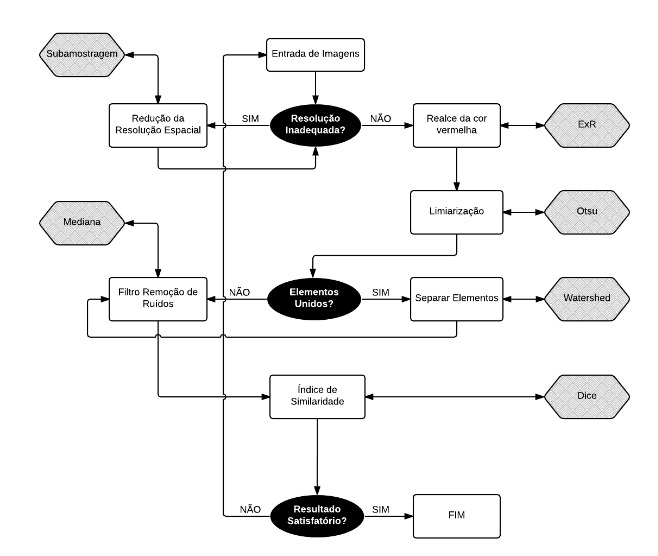
\includegraphics[width=1\textwidth]{./dados/figuras/pipeline-paglione.jpeg}
    \fonte{}
    \label{fig:figura-pipelinePreProcessamento}
\end{figure}

A aquisição das imagens é dada a partir da base de dados composta por lâminas de sementes de soja. A primeiro momento é verificado a resolução das imagens de entrada, caso seja inapropriadamente alta, está será reduzida utilizando o método \textit{downsampling}.

\subsection{PRÉ-PROCESSAMENTO}
\label{sec:titSubSecPreProcessamento}

Como descrito na \autoref{sec:titSecAnalSementes}, a solução do teste de tetrazólio proporciona uma cor avermelhada as sementes de soja submetidas, e está cor caracteriza o resultado do teste. Em função disso, será realçada a cor vermelha, para melhor proveito do conceito de índice de vegetação ExR, excesso de vermelho (do inglês, \textit{Excess Red}), a fim de uma melhor análise dos resultados. E então realizada uma limiarização de Otsu, com o objetivo de segmentar as imagens de semente de soja do fundo, proporcionando uma cor branca as sementes e ao fundo da imagem, a cor preta. Caso a imagem resultante ainda conter elementos conectados entre si é aplicado o algoritmo de segmentação de \textit{watershed}. E por fim, aplicado o filtro de mediana para remoção de possíveis ruídos.

Para a etapa de representação e descrição será utilizado um \textit{script} desenvolvido na linguagem python que agrupará as imagens em \textit{clusters} semelhantes utilizando-se técnicas de aprendizado de máquina, além do auxílio da API Keras. A Keras é uma biblioteca de \textit{Deep Learning} de alto nível desenvolvida em python, capaz de executar em uma camada acima da TensorFlow - biblioteca de código aberto para aprendizado de máquina, desenvolvida pela Google. A biblioteca dispõe de modelos de aprendizado profundo, pré-treinados por imagens da ImageNet, que serão utilizados para extração de um vetor com as características das imagens.

\subsection{FLORESTA DE CAMINHOS ÓTIMOS}
\label{sec:titSubSecOPF}

A etapa de reconhecimento e interpretação, como citado anteriormente na \autoref{sec:titSecVisaoComputacional}, envolve a realização de aprendizado e representar os padrões aprendidos. Para isso, este trabalho tem como objetivo propor e desenvolver uma nova técnica de aprendizado supervisionado por meio de variáveis latentes. Para tanto, a mesma será baseada no conceito de Floresta de Caminhos Ótimos (OPF, do inglês \textit{Optimum Path Forest}), o qual apresenta resultados eficazes e eficientes quando comparado com outros algoritmos de aprendizado supervisionado da literatura (PAPA, 2008).

As florestas de caminhos ótimos embasam-se no conceito de otimização de caminhos por meio do algoritmo de Dijkstra
contendo múltiplas fontes e sumidouros. Dessa forma, o classificador supervisionado OPF consiste em um arcabouço para instanciação de classificadores baseados nas florestas de caminhos ótimos. Os métodos de aprendizado suportados por tal arcabouço são o supervisionado e o não-supervisionado, neste trabalho foi utilizado o método de aprendizado supervisionado com uma abordagem de grafo completo.

Vale ressaltar que, a maioria dos classificadores na literatura geralmente apresentam boa eficácia a partir de um grande conjunto de dados de treinamento, já a OPF mostrou-se eficaz, na maioria das vezes, bem como eficiente em treinamentos e testes independentemente do tamanho do conjunto de dados. 

Após as \textit{deep features} serem extraídas das imagens as mesmas foram organizadas em vetores de características. A OPF modela cada vetor como sendo um nó de um grafo completo, ou seja, todos os nós devem estar conectados. O algoritmo de treinamento encarrega-se de escolher os protótipos de cada classe (raízes de cada árvore de caminho ótimo). Esses, por sua vez, tentarão conquistar os outros nós não-protótipos. Um custo é atribuído a cada nó não-protótipo e a aresta que apresentar o menor custo entre o nó protótipo, conquista a amostra atribuindo a essa o rótulo da classe.

Os passos realizados pela abordagem proposta são explicitados na Figura 3. No passo 1, todas as amostras são conectadas e definidos os protótipos de cada classe (ilustrados pela borda pontilhada), em seguida é calculado o peso de cada aresta. Para cada nó é definido também uma função de custo, após isso os nós protótipos irão tentar conquistar as demais amostras, o protótipo que oferecer o menor custo à outra amostra, conquista a amostra. No passo 2, é ilustrado o processo após o treinamento, onde o
protótipo A conquistou a amostra B e o protótipo C conquistou a amostra D. No passo 3, é ilustrado a fase de teste, onde uma nova amostra teste será conectada aos demais nós da rede e essa será conquistada pela amostra que lhe oferecer o menor custo, na
Figura 3 temos que a amostra X será conquistada pelo nó A.

\begin{figure}[!htb]
    \centering
    \caption{Fase de teste da OPF}
    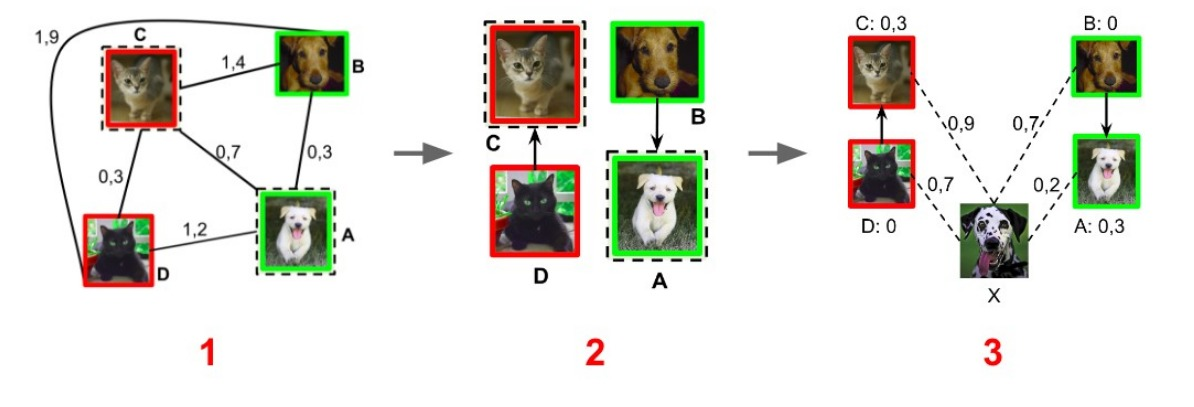
\includegraphics[width=1\textwidth]{./dados/figuras/opf-funcionamento.jpeg}
    \fonte{Autoria própria}
    \label{fig:figura-FaseTesteOPF}
\end{figure}

\subsection{ANÁLISE DE VARIÁVEIS LATENTES}
\label{sec:titSubSecVarLatentes}

Uma variável latente auxilia no fato de que não é necessário comparar inúmeras correlações para encontrar padrões, empregando apenas algumas técnicas estatísticas é possível inferir padrões (ANDRADE et al., 2014).

Para realizar a identificação de variáveis latentes no contexto de análise de imagens foi então utilizado o conceito de floresta de caminhos ótimos, o qual calcula a distância entre cada nó da etapa de treinamento e teste. Dessa forma, a partir de tais informações pôde-se utilizar tais distâncias para propor e calcular uma formulação para pertinência de cada sub-imagem a cada uma das classes abordadas em um dado contexto. A partir de tal formulação é possível obter relevância de uma dada amostra (i.e. sub-imagem) pertencer ou não às classes abordadas no problema. Tal informação é obtida facilmente por meio do menor valor correspondente na lista de distâncias, representada por h+, e menor valor com classe diferente da sub-imagem na lista de distâncias, denotada por h-. A pontuação é dada a partir da \autoref{eq:equacao-score}.

\begin{equation}
    score = |\, ({h}^{+}) \, - \, ({h}^{-}) \, |
    \label{eq:equacao-score}
\end{equation}

As pontuações de todas as sub imagens são armazenadas e comparadas, com o intuito de identificar quais fragmentos da imagem original obtiveram maior e menor pontuação. Sendo possível obter as variáveis latentes, dada a maior e menor pontuações.

\section{RESULTADOS ESPERADOS}
\label{sec:titSecResultEsperados}

Espera-se desenvolver uma técnica capaz de realizar o aprendizado
profundo de máquina, solucionando o erro de mapeamento dos classificadores atuais, empregando métodos e os respectivos passos que foram descritos na \autoref{sec:titSecMetProposta}.

Analisar qual o método mais eficiente da biblioteca Keras, para extração de características, que trará os melhores resultados. E analisar a eficiência da biblioteca da OPF e quais parâmetros permitem desenvolver um classificador que retorne os resultados esperado para o teste de tetrazólio.

Entender, por meio das variáveis latentes, quais fatores desencadeiam uma classificação equivocada, para a base de imagens utilizada.

Obter bons resultados que permitam que o classificador atenda as expectativas humanas no teste de tetrazólio.

                   % Metodologia
% RESULTADOS-------------------------------------------------------------------

\chapter{ANÁLISE E DISCUSSÃO DOS RESULTADOS}

Cada capítulo deve conter uma pequena introdução (tipicamente, um ou dois parágrafos) que deve deixar claro o objetivo e o que será discutido no capítulo, bem como a organização do capítulo.
                    % Resultados
% ORIENTAÇÕES GERAIS------------------------------------------------------------


% SOBRE AS ILUSTRAÇÕES----------------------------------------------------------
\chapter{SOBRE AS ILUSTRAÇÕES}
\label{chap:apSobreIlust}

A seguir exemplifica-se como inserir ilustrações no corpo do trabalho. As ilustrações serão indexadas automaticamente em suas respectivas listas. A numeração sequencial de figuras, tabelas e equações também ocorre de modo automático.

Referências cruzadas são obtidas através dos comandos \verb|\label{}| e \verb|\ref{}|. Sendo assim, não é necessário por exemplo, saber que o número de certo capítulo é \ref{chap:fundamentacaoTeorica} para colocar o seu número no texto. Outra forma que pode ser utilizada é esta: \autoref{chap:fundamentacaoTeorica}, facilitando a inserção, remoção e manejo de elementos numerados no texto sem a necessidade de renumerar todos esses elementos.

% FIGURAS-----------------------------------------------------------------------
\chapter{FIGURAS}
\label{chap:figuras}

Exemplo de como inserir uma figura. A \autoref{fig:figura-exemplo1} aparece automaticamente na lista de figuras. Para saber mais sobre o uso de imagens no \LaTeX{} consulte literatura especializada \cite{Goossens2007}.

Os arquivos das figuras devem ser armazenados no diretório de "/dados".

\begin{figure}[!htb]
    \centering
    \caption{Exemplo de Figura}
    \includegraphics[width=0.5\textwidth]{./dados/figuras/figura1}
    \fonte{\citeonline{}}
    \label{fig:figura-exemplo1}
\end{figure}

% QUADROS E TABELAS---------------------------------------------------------------
\chapter{QUADROS E TABELAS}
\label{chap:tabelas}

Exemplo de como inserir o \autoref{qua:quadro-exemplo1} e a \autoref{tab:tabela-exemplo1}. Ambos aparecem automaticamente nas suas respectivas listas. Para saber mais informações sobre a construção de tabelas no \LaTeX{} consulte literatura especializada \cite{Mittelbach2004}.

Ambos os elementos (Quadros e Tabelas) devem ser criados em arquivos separados para facilitar manutenção e armazenados no diretório de "/dados".

\begin{quadro}[!htb]
    \centering
    \caption{Exemplo de Quadro.\label{qua:quadro-exemplo1}}
    \begin{tabular}{|p{7cm}|p{7cm}|}
        \hline
        \textbf{BD Relacionais} & \textbf{BD Orientados a Objetos} \\
        \hline
        Os dados são passivos, ou seja, certas operações limitadas podem ser automaticamente acionadas quando os dados são usados. Os dados são ativos, ou seja, as solicitações fazem com que os objetos executem seus métodos. & Os processos que usam dados mudam constantemente. \\
        \hline
    \end{tabular}
    \fonte{\citeonline{Barbosa2004}}
\end{quadro}


A diferença entre quadro e tabela está no fato que um quadro é formado por linhas horizontais e verticais. Deve ser utilizado quando o conteúdo é majoritariamente não-numérico. O número do quadro e o título vem acima do quadro, e a fonte, deve vir abaixo. E Uma tabela é formada apenas por linhas verticais. Deve ser utilizada quando o conteúdo é majoritariamente numérico. O número da tabela e o título vem acima da tabela, e a fonte, deve vir abaixo, tal como no quadro.

\begin{table}[!htb]
    \centering
    \caption[Resultado dos testes]{Resultado dos testes.
    \label{tab:tabela-exemplo1}}
    \begin{tabular}{rrrrr}
        \toprule
            & Valores 1 & Valores 2 & Valores 3 & Valores 4 \\
        \midrule
            Caso 1 & 0,86 & 0,77 & 0,81 & 163 \\
            Caso 2 & 0,19 & 0,74 & 0,25 & 180 \\
            Caso 3 & 1,00 & 1,00 & 1,00 & 170 \\
        \bottomrule
    \end{tabular}
    \fonte{\citeonline{Barbosa2004}}
\end{table}


% EQUAÇÕES-----------------------------------------------------------------------
\chapter{EQUAÇÕES}
\label{chap:equacoes}

Exemplo de como inserir a \autoref{eq:equacao-exemplo1} e a Eq. \ref{eq:equacao-exemplo2} no corpo do texto \footnote{Deve-se atentar ao fato de a formatação das equações ficar muito boa esteticamente.}. Observe que foram utilizadas duas formas distintas para referenciar as equações.

\begin{equation}
    X(s) = \int\limits_{t = -\infty}^{\infty} x(t) \, \text{e}^{-st} \, dt
    \label{eq:equacao-exemplo1}
\end{equation}

\begin{equation}
    F(u, v) = \sum_{m = 0}^{M - 1} \sum_{n = 0}^{N - 1} f(m, n) \exp \left[ -j 2 \pi \left( \frac{u m}{M} + \frac{v n}{N} \right) \right]
    \label{eq:equacao-exemplo2}
\end{equation}

% ALGORITMOS-----------------------------------------------------------------------
\chapter{ALGORITMOS}
\label{chap:algoritmos}

Exemplo de como inserir um algoritmo. Para inserção de algoritmos utiliza-se o pacote {\ttfamily algorithm2e} que já está devidamente configurado dentro do template.

Os algoritmos devem ser criados em arquivos separados para facilitar manutenção e armazenados no diretório de "/dados".\\
\\

\begin{algorithm}
    \caption{Exemplo de Algoritmo}
    \KwIn{o número $n$ de vértices a remover, grafo original $G(V, E)$}
    \KwOut{grafo reduzido $G'(V,E)$}
    $removidos \leftarrow 0$ \\
    \While {removidos $<$ n } {
        $v \leftarrow$ Random$(1, ..., k) \in V$ \\
            \For {$u \in adjacentes(v)$} {
                remove aresta (u, v)\\
                $removidos \leftarrow removidos + 1$\\
            }
            \If {há  componentes desconectados} {
                remove os componentes desconectados\\
            }
        }
\end{algorithm}


% SOBRE AS LISTAS--------------------------------------------------------------------
\chapter{SOBRE AS LISTAS}
\label{chap:apSobreLista}

Para construir listas de "\textit{bullets}"{} ou listas enumeradas, inclusive listas aninhadas, é utilizado o pacote \verb|paralist|.

Exemplo de duas listas não numeradas aninhadas, utilizando o comando \verb|\itemize|. Observe a indentação, bem como a mudança automática do tipo de "\textit{bullet}"{} nas listas aninhadas.

\begin{itemize}
    \item item não numerado 1
    \item item não numerado 2
    \begin{itemize}
        \item subitem não numerado 1
        \item subitem não numerado 2
        \item subitem não numerado 3
    \end{itemize}
    \item item não numerado 3
\end{itemize}

Exemplo de duas listas numeradas aninhadas, utilizando o comando \verb|\enumerate|. Observe a numeração progressiva e indentação das listas aninhadas.

\begin{enumerate}
    \item item numerado 1
    \item item numerado 2
    \begin{enumerate}
        \item subitem numerado 1
        \item subitem numerado 2
        \item subitem numerado 3
    \end{enumerate}
    \item item numerado 3
\end{enumerate}

% SOBRE AS CITAÇÕES E CHAMADAS DE REFERÊNCAS----------------------------------------------
\chapter{SOBRE AS CITAÇÕES E CHAMADAS DE REFERÊNCAS}
\label{chap:apSobreCita}

Citações são trechos de texto ou informações obtidas de materiais consultadss quando da elaboração do trabalho. São utilizadas no texto com o propósito de esclarecer, completar e embasar as ideias do autor. Todas as publicações consultadas e utilizadas (por meio de citações) devem ser listadas, obrigatoriamente, nas referências bibliográficas, para preservar os direitos autorais. São classificadas em citações indiretas e diretas.

% CITAÇÕES INDIRETAS-----------------------------------------------------------------------
\chapter{CITAÇÕES INDIRETAS}
\label{chap:citacoesLivres}

É a transcrição, com suas próprias palavras, das idéias de um autor, mantendo-se o sentido original. A citação indireta é a maneira que o pesquisador tem de ler, compreender e gerar conhecimento a partir do conhecimento de outros autores. Quanto à chamada da referência, ela pode ser feita de duas maneiras distintas, conforme o nome do(s) autor(es) façam parte do seu texto ou não. Exemplo de chamada fazendo parte do texto:\\
\\Enquanto \citeonline{Maturana2003} defendem uma epistemologia baseada na biologia. Para os autores, é necessário rever \ldots.\\

A chamada de referência foi feita com o comando \verb|\citeonline{chave}|, que produzirá a formatação correta.

A segunda forma de fazer uma chamada de referência deve ser utilizada quando se quer evitar uma interrupção na sequência do texto, o que poderia, eventualmente, prejudicar a leitura. Assim, a citação é feita e imediatamente após a obra referenciada deve ser colocada entre parênteses. Porém, neste caso específico, o nome do autor deve vir em caixa alta, seguido do ano da publicação. Exemplo de chamada não fazendo parte do texto:\\
\\Há defensores da epistemologia baseada na biologia que argumentam em favor da necessidade de \ldots \cite{Maturana2003}.\\

Nesse caso a chamada de referência deve ser feita com o comando \verb|\cite{chave}|, que produzirá a formatação correta.

% CITAÇÕES DIRETAS-----------------------------------------------------------------------
\chapter{CITAÇÕES DIRETAS}
\label{chap:citacoesLiterais}

É a transcrição ou cópia de um parágrafo, de uma frase, de parte dela ou de uma expressão, usando exatamente as mesmas palavras adotadas pelo autor do trabalho consultado.

Quanto à chamada da referência, ela pode ser feita de qualquer das duas maneiras já mencionadas nas citações indiretas, conforme o nome do(s) autor(es) façam parte do texto ou não. Há duas maneiras distintas de se fazer uma citação direta, conforme o trecho citado seja longo ou curto.

Quando o trecho citado é longo (4 ou mais linhas) deve-se usar um parágrafo específico para a citação, na forma de um texto recuado (4 cm da margem esquerda), com tamanho de letra menor e espaçamento entrelinhas simples. Exemplo de citação longa:
\\\begin{citacao}
    Desse modo, opera-se uma ruptura decisiva entre a reflexividade filosófica, isto é a possibilidade do sujeito de pensar e de refletir, e a objetividade científica. Encontramo-nos num ponto em que o conhecimento científico está sem consciência. Sem consciência moral, sem consciência reflexiva e também subjetiva. Cada vez mais o desenvolvimento extraordinário do conhecimento científico vai tornar menos praticável a própria possibilidade de reflexão do sujeito sobre a sua pesquisa \cite[p.~28]{Silva2000}.
\end{citacao}

Para fazer a citação longa deve-se utilizar os seguintes comandos:
\begin{verbatim}
\begin{citacao}
<texto da citacao>
\end{citacao}
\end{verbatim}

No exemplo acima, para a chamada da referência o comando \verb|\cite[p.~28]{Silva2000}| foi utilizado, visto que os nomes dos autores não são parte do trecho citado. É necessário também indicar o número da página da obra citada que contém o trecho citado.

Quando o trecho citado é curto (3 ou menos linhas) ele deve inserido diretamente no texto entre aspas. Exemplos de citação curta:\\
\\A epistemologia baseada na biologia parte do princípio de que "assumo que não posso fazer referência a entidades independentes de mim para construir meu explicar" \cite[p.~35]{Maturana2003}.\\
\\A epistemologia baseada na biologia de \citeonline[p.~35]{Maturana2003} parte do princípio de que "assumo que não posso fazer referência a entidades independentes de mim para construir meu explicar".

% DETALHES SOBRE AS CHAMADAS DE REFERÊNCIAS---------------------------------------------------------
\chapter{DETALHES SOBRE AS CHAMADAS DE REFERÊNCIAS}
\label{chap:referUtilizadas}

Outros exemplos de comandos para as chamadas de referências e o resultado produzido por estes:\\
\\\citeonline{Maturana2003} \ \ \  \verb|\citeonline{Maturana2003}|\\
\citeonline{Barbosa2004} \ \ \   \verb|\citeonline{Barbosa2004}|\\
\cite[p.~28]{Silva2000} \ \ \  \verb|\cite[p.~28]{Silva2000}|\\
\citeonline[p.~33]{Silva2000} \ \ \   \verb|\citeonline[p.~33]{v}|\\
\cite[p.~35]{Maturana2003} \ \ \   \verb|\cite[p.~35]{Maturana2003}|\\
\citeonline[p.~35]{Maturana2003} \ \ \   \verb|\citeonline[p.~35]{Maturana2003}|\\
\cite{Barbosa2004,Maturana2003} \ \ \   \verb|\cite{Barbosa2004,Maturana2003}|\\

% SOBRE AS REFERÊNCIAS BIBLIOGRÁFICAS-------------------------------------------------------
\chapter{SOBRE AS REFERÊNCIAS BIBLIOGRÁFICAS}
\label{chap:apSobreRefer}

A bibliografia é feita no padrão \textsc{Bib}\TeX{}. As referências são colocadas em um arquivo separado. Neste template as referências são armazenadas no arquivo "base-referencias.bib".

Existem diversas categorias documentos e materiais componentes da bibliografia. A classe abn\TeX{} define as seguintes categorias (entradas):

\begin{verbatim}
@book
@inbook
@article
@phdthesis
@mastersthesis
@monography
@techreport
@manual
@proceedings
@inproceedings
@journalpart
@booklet
@patent
@unpublished
@misc
\end{verbatim}

Cada categoria (entrada) é formatada pelo pacote \citeonline{abnTeX22014d} de uma forma específica. Algumas entradas foram introduzidas especificamente para atender à norma \citeonline{NBR6023:2002}, são elas: \verb|@monography|, \verb|@journalpart|,\verb|@patent|. As demais entradas são padrão \textsc{Bib}\TeX{}. Para maiores detalhes, refira-se a \citeonline{abnTeX22014d}, \citeonline{abnTeX22014b}, \citeonline{abnTeX22014c}.

% NOTAS DE RODAPÉ--------------------------------------------------------------------------
\chapter{NOTAS DE RODAPÉ}
\label{chap:notasRodape}

As notas de rodapé pode ser classificadas em duas categorias: notas explicativas\footnote{é o tipo mais comum de notas que destacam, explicam e/ou complementam o que foi dito no corpo do texto, como esta nota de rodapé, por exemplo.} e notas de referências. A notas de referências, como o próprio nome ja indica, são utilizadas para colocar referências e/ou chamadas de referências sob certas condições.
                   % Capítulo com Orientações de uso do Template
% CONCLUSÃO--------------------------------------------------------------------

\chapter{CONCLUSÃO}
\label{chap:conclusao}

Parte final do texto, na qual se apresentam as conclusões do trabalho acadêmico. É importante fazer uma análise crítica do trabalho, destacando os principais resultados e as contribuições do trabalho para a área de pesquisa.

\section{TRABALHOS FUTUROS}
\label{sec:trabalhosFuturos}

Também deve indicar, se possível e/ou conveniente, como o trabalho pode ser estendido ou aprimorado.

\section{CONSIDERAÇÕES FINAIS}
\label{sec:consideracoesFinais}

Encerramento do trabalho acadêmico.
                 			   % Conclusão

\postextual
% INSERE ELEMENTOS PÓS-TEXTUAIS
% REFERÊNCIAS------------------------------------------------------------------

% Carrega o arquivo "base-referencias.bib" e extrai automaticamente as referências citadas

\bibliography{./base-referencias}
\bibliographystyle{abntex2-alf} % Define o estilo ABNT para formatar a lista de referências
% OBSERVAÇÕES------------------------------------------------------------------
% Este arquivo não precisa ser alterado.
           			   % Referências
% APÊNDICES--------------------------------------------------------------------

\begin{apendicesenv}
\partapendices

% Primeiro apêndice------------------------------------------------------------
\chapter{Nome do apêndice} % Edite para alterar o título deste apêndice
\label{chap:apendiceA}

Lembre-se que a diferença entre apêndice e anexo diz respeito à autoria do texto e/ou material ali colocado.

Caso o material ou texto suplementar ou complementar seja de sua autoria, então ele deverá ser colocado como um apêndice. Porém, caso a autoria seja de terceiros, então o material ou texto deverá ser colocado como anexo.

Caso seja conveniente, podem ser criados outros apêndices para o seu trabalho acadêmico. Basta recortar e colar este trecho neste mesmo documento. Lembre-se de alterar o "label"{} do apêndice.

Não é aconselhável colocar tudo que é complementar em um único apêndice. Organize os apêndices de modo que, em cada um deles, haja um único tipo de conteúdo. Isso facilita a leitura e compreensão para o leitor do trabalho.

% Novo apêndice----------------------------------------------------------------
\chapter{Nome do outro apêndice}
\label{chap:apendiceB}

conteúdo do novo apêndice

\end{apendicesenv}
             			   % Apêndices
% ANEXO------------------------------------------------------------------------

\begin{anexosenv}
\partanexos

% Primeiro anexo---------------------------------------------------------------
\chapter{Nome do anexo}     % edite para alterar o título deste anexo
\label{chap:anexoA}

Lembre-se que a diferença entre apêndice e anexo diz respeito à autoria do texto e/ou material ali colocado.

Caso o material ou texto suplementar ou complementar seja de sua autoria, então ele deverá ser colocado como um apêndice. Porém, caso a autoria seja de terceiros, então o material ou texto deverá ser colocado como anexo.

Caso seja conveniente, podem ser criados outros anexos para o seu trabalho acadêmico. Basta recortar e colar este trecho neste mesmo documento. Lembre-se de alterar o "label"{} do anexo.

Organize seus anexos de modo a que, em cada um deles, haja um único tipo de conteúdo. Isso facilita a leitura e compreensão para o leitor do trabalho. É para ele que você escreve.

% Novo anexo-------------------------------------------------------------------
\chapter{Nome do outro anexo}
\label{chap:anexoB}

conteúdo do outro anexo

\end{anexosenv}
               			   % Anexos

\end{document}
